\documentclass[titlepage]{article}

\usepackage{graphicx}
\usepackage{lastpage}
\usepackage{fancyhdr}
\usepackage{hyperref}
\usepackage{amsmath}
\usepackage{tcolorbox}
\usepackage{makecell}
\usepackage{cancel}
\usepackage{geometry}
\usepackage{listings}

\definecolor{vgreen}{RGB}{104,180,104}
\definecolor{vblue}{RGB}{49,49,255}
\definecolor{vorange}{RGB}{255,143,102}

\lstdefinestyle{verilog-style}
{
    language=Verilog,
    basicstyle=\small\ttfamily,
    keywordstyle=\color{vblue},
    identifierstyle=\color{black},
    commentstyle=\color{vgreen},
    numbers=left,
    numberstyle=\tiny\color{black},
    numbersep=10pt,
    tabsize=8,
    moredelim=*[s][\colorIndex]{[}{]},
    literate=*{:}{:}1
}
\makeatletter
\newcommand*\@lbracket{[}
\newcommand*\@rbracket{]}
\newcommand*\@colon{:}
\newcommand*\colorIndex{%
    \edef\@temp{\the\lst@token}%
    \ifx\@temp\@lbracket \color{black}%
    \else\ifx\@temp\@rbracket \color{black}%
    \else\ifx\@temp\@colon \color{black}%
    \else \color{vorange}%
    \fi\fi\fi
}
\makeatother



\hypersetup{
    colorlinks=true,
    linkcolor=blue, 
    filecolor=magenta,
    urlcolor=blue
}

\setcounter{secnumdepth}{0}

\pagestyle{fancy}
\fancyhf{}
\renewcommand{\headrulewidth}{0pt}
\rfoot{\thepage \hspace{1pt} of \pageref{LastPage}}

\begin{document}


\begin{titlepage}
    \begin{center}
        \Huge
        \vspace*{3cm}
        \textbf{  ADVD \\  \quad Assignment 1} \\
        \quad EEE F313\\[3ex]
        \huge
        \quad Problem set 72 \\[2ex]
        \quad\includegraphics[scale=0.75]{BITS_Pilani-Logo.png}
        \vfill
        \huge
        \quad Sai Kartik (2020A3PS0435P)\\\quad Rajeev Rajagopal (2020A3PS1237P) \\ \quad Manpreet Singh (2020A3PS0419P)
    \end{center}
\end{titlepage}

\newgeometry{left=2cm,bottom=2cm,right=2cm,top=2cm}

\pagenumbering{roman}

\tableofcontents
\listoffigures
\newpage
\pagenumbering{arabic}
\setcounter{page}{1}

\section {Problem 1}

\begin{tcolorbox}
    Design a 4:1 multiplexer using CMOS logic style. Simulate with a 500fF load capacitance
\end{tcolorbox}

\subsection{Solution}

\subsubsection{Schematic design}
The schematic design is shown below
\begin{figure}[ht]
    \centering
    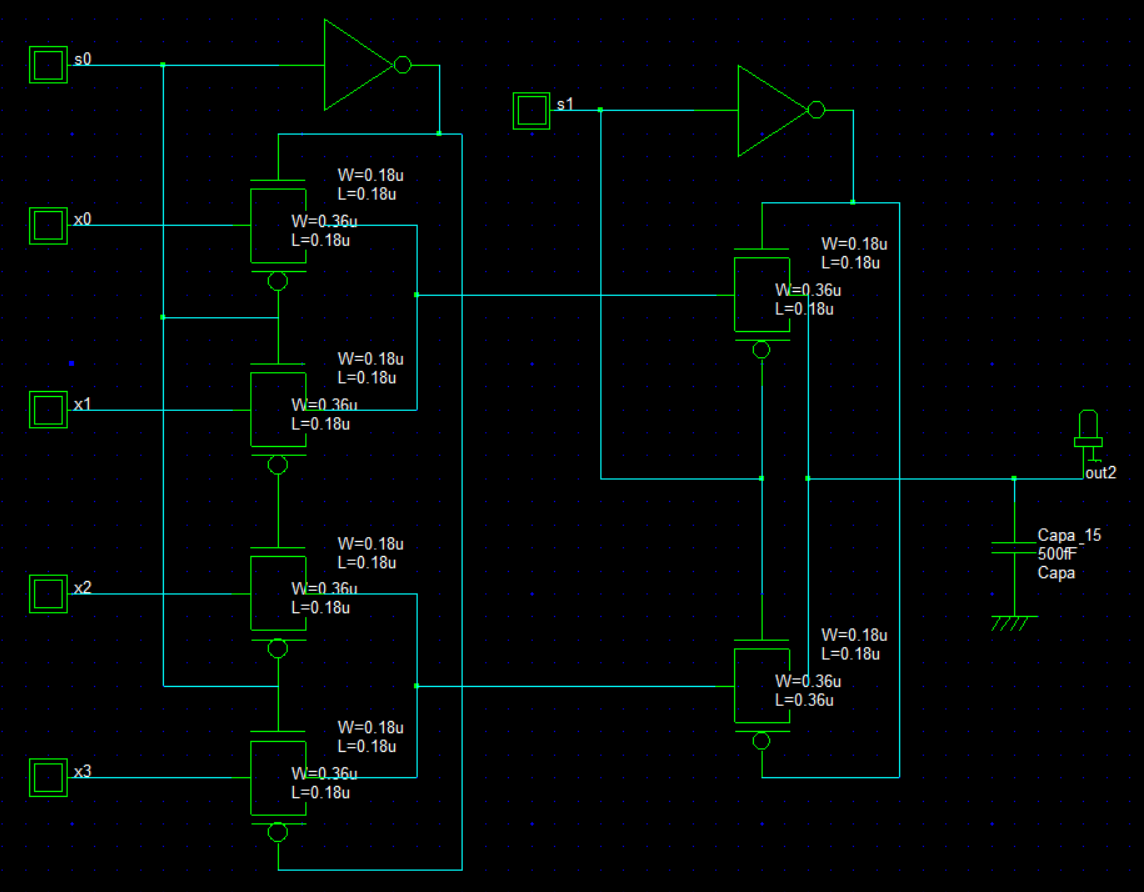
\includegraphics[scale = 0.5]{muxsch.png}
    \caption{Schematic design for a 4:1 mux using transmission gates}
    \label{fig1}
\end{figure}
\newpage
\subsubsection{Layout design}
Since we're using the cmos018.rul library, we have the value of $L$ as 180nm. We chose the value of $W/L$ as 1 for all NMOS and 2 for all PMOS. This implies the value for $W$ and $L$ for NMOS is 180nm. $W$ and $L$ values for PMOS is 360nm and 180nm respectively. The layout design is shown below.
\begin{figure}[ht]
    \centering
    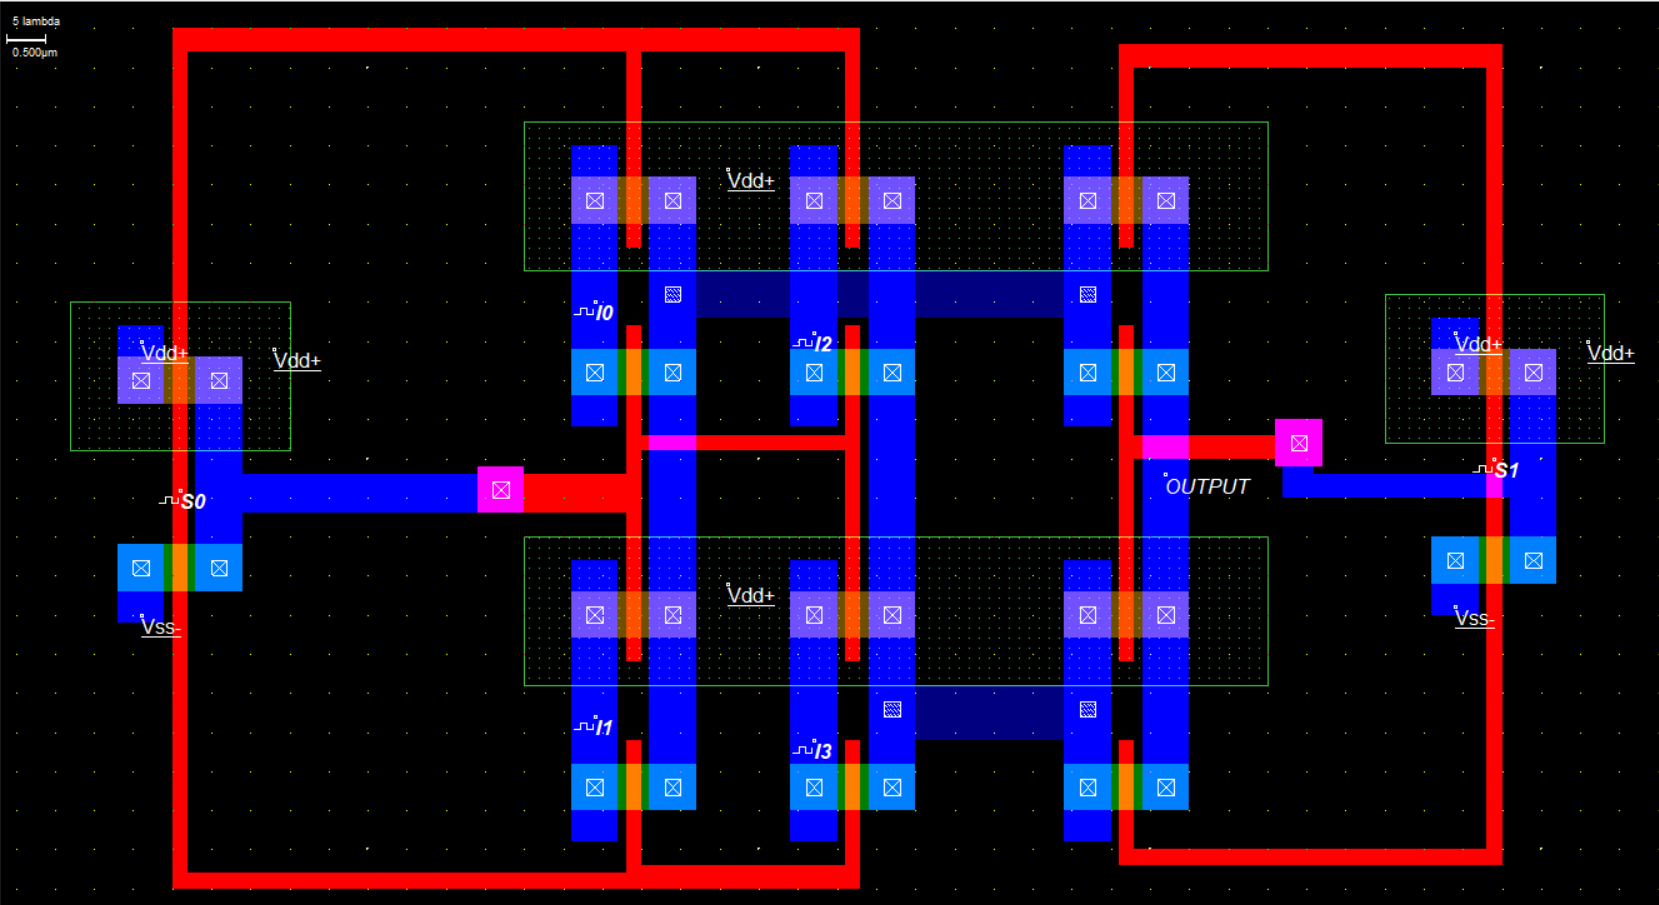
\includegraphics[scale = 0.50]{Layout_Ass1a.png}
    \caption{Layout design}
    \label{fig2}
\end{figure}
\paragraph*{Reasoning}
From the spice netlist of the circuit we found that the value of $\mu_n$ and $\mu_p$ were 380 and 200 units respectively. Equating $\mu_nC_{ox}\frac WL$ of NMOS to $\mu_p C_{ox}\frac WL$ of PMOS and keeping the value of $L$ constant for both PMOS and NMOS at 180nm, we came to the relation of $\frac{W_p}{W_n} = 1.9 \approx 2$. This is why the value of $W$ for PMOS is taken to be 360nm and $W$ for NMOS is taken to be 180nm.
\newpage

\newpage
\subsubsection{Area, power consumption and delays}
\paragraph*{Area of the layout}
As per the statistics generated by Microwind, the area of the layout is $23.4 \mu \text{m} \times 11.0 \mu \text{m} = 257.4 \mu \text{m}^2$
\begin{figure}[ht]
    \centering
    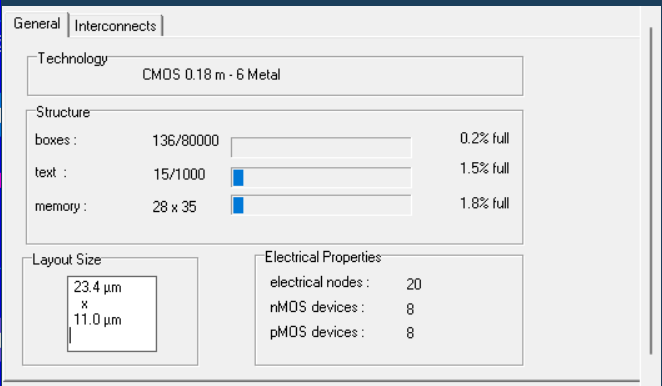
\includegraphics{area.png}
    \caption{Area of the layout}
\end{figure}
\paragraph*{Power consumption}
As per the graph below, the power consumed by circuit comes out to be 71.904$\mu$W. \newline
\begin{figure}[ht]
    \centering
    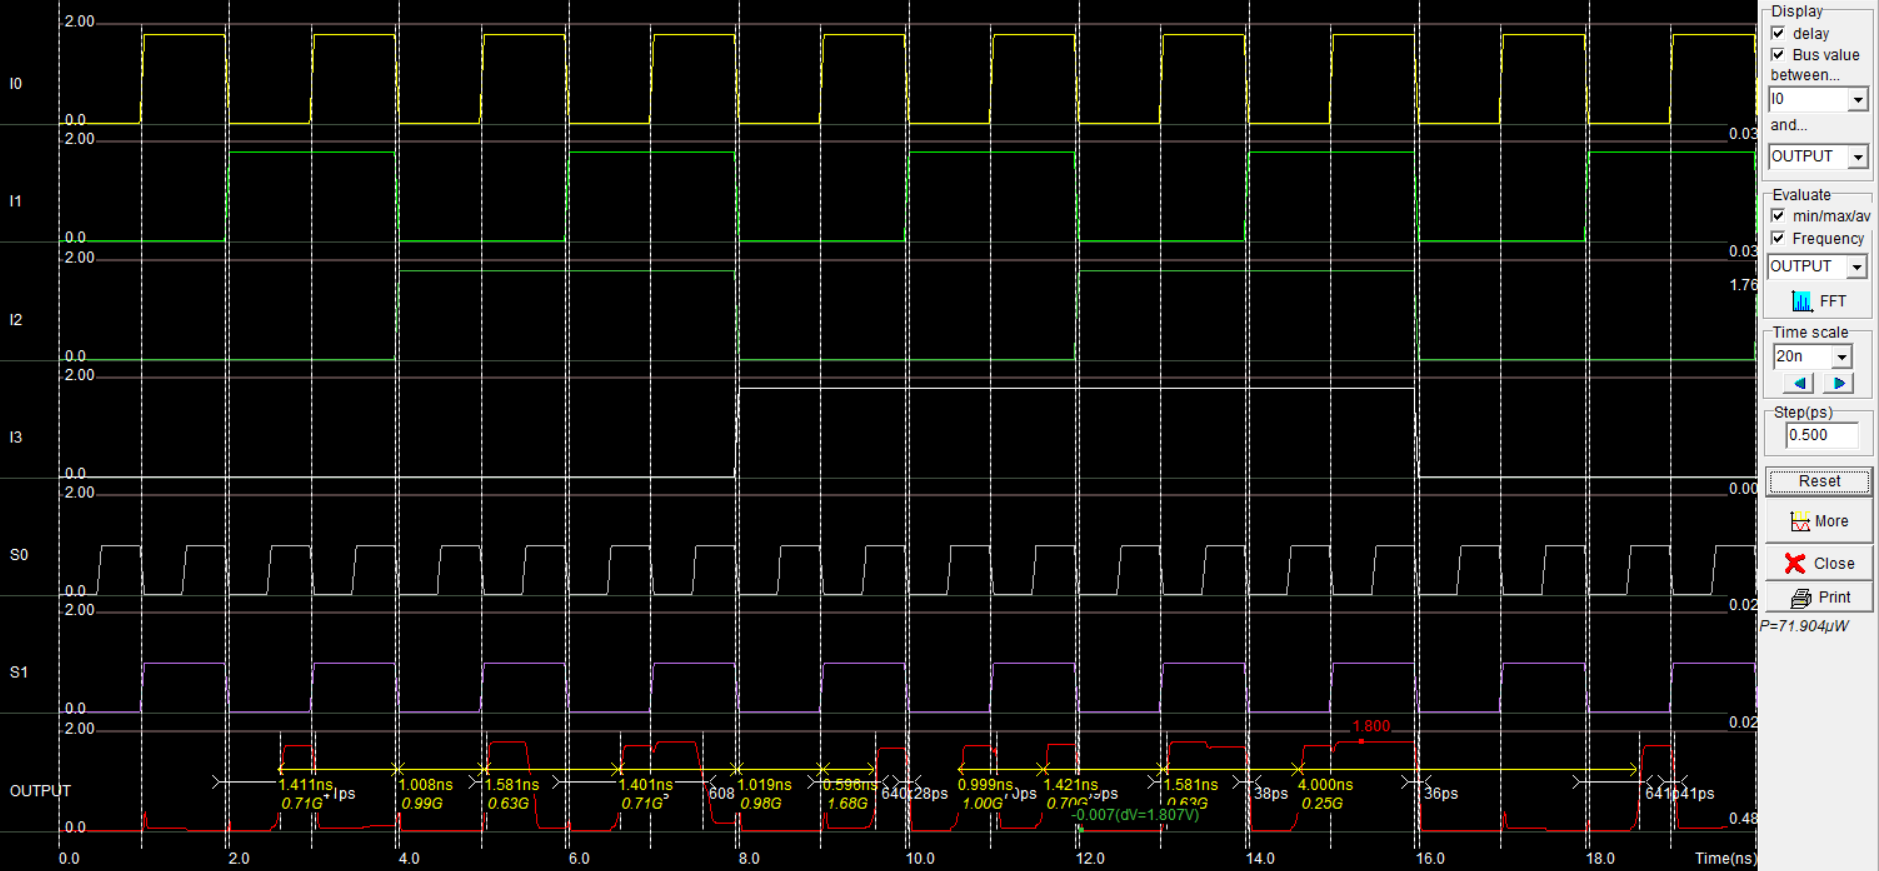
\includegraphics[scale = 0.4]{Voltvstime_Ass1a.png}
    \caption{Voltage vs time graph}
\end{figure}
\clearpage
\paragraph*{Delay calculation}
The average propagation delay calculated is 0.164ns.
\begin{figure}[ht]
    \centering
    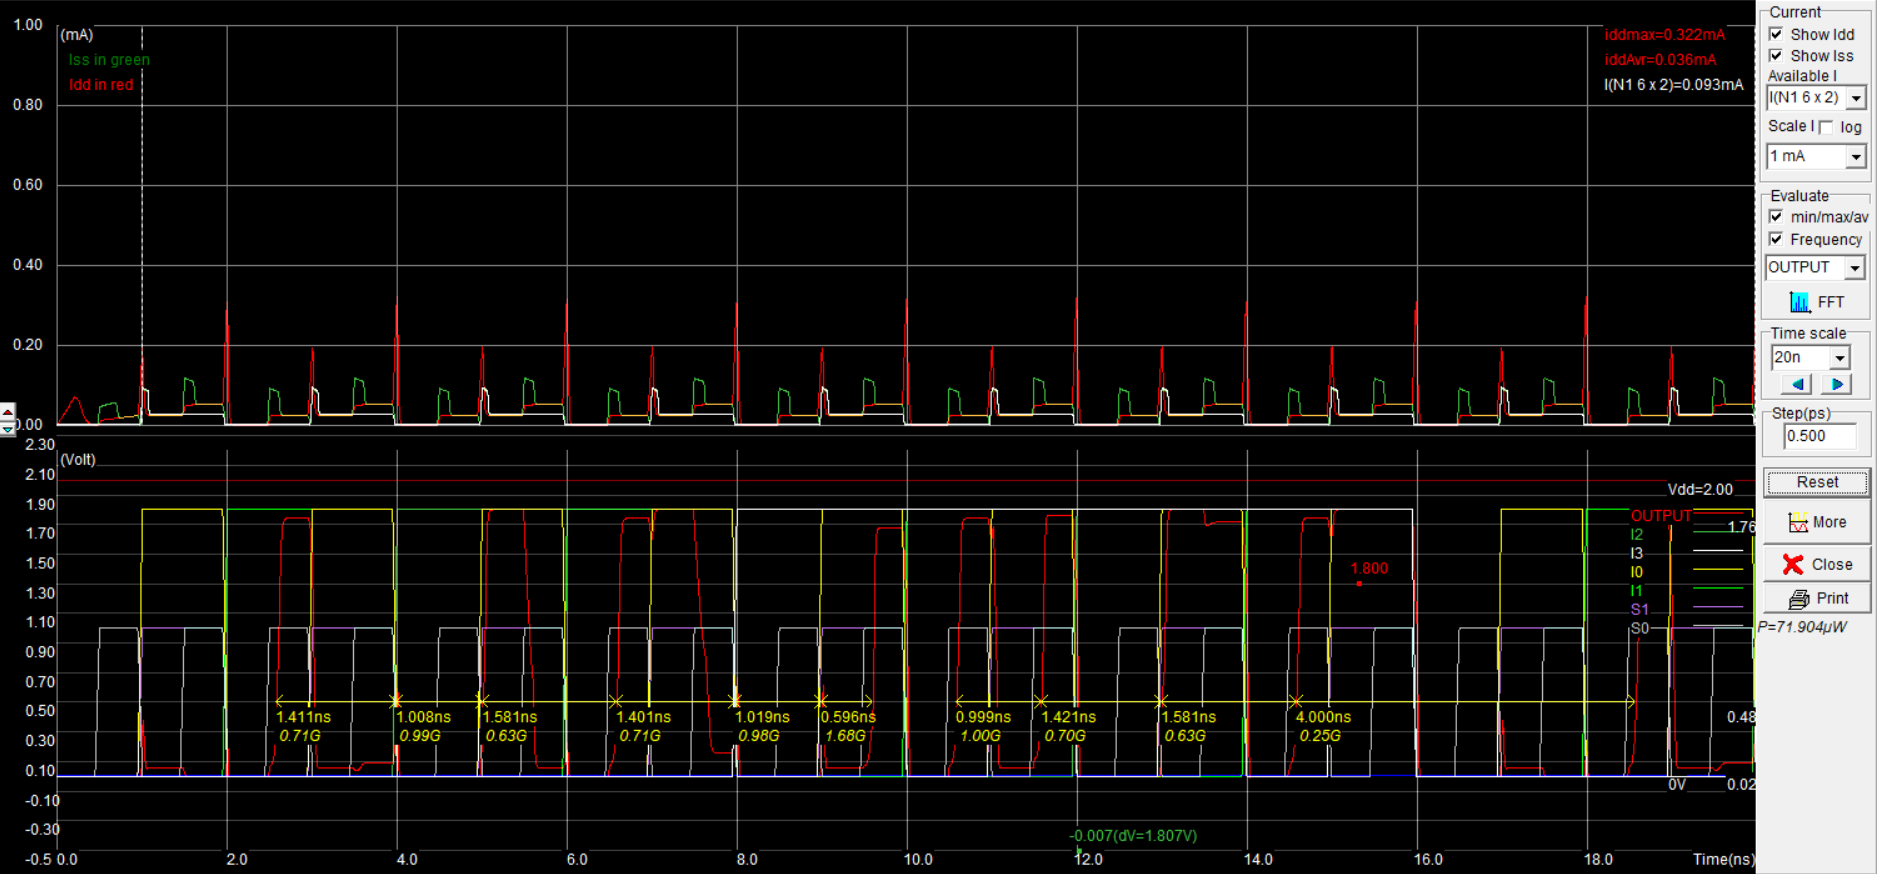
\includegraphics[scale = 0.4]{voltandcurrent_Ass1a.png}
    \caption{Voltage vs time and current vs time graphs}
\end{figure}

\subsubsection{Layout design generated by Microwind}
Corresponding to the verilog file generated for the schematic shown in Figure \ref{fig1}, Microwind has generated the following layout
\begin{figure}[ht]
    \centering
    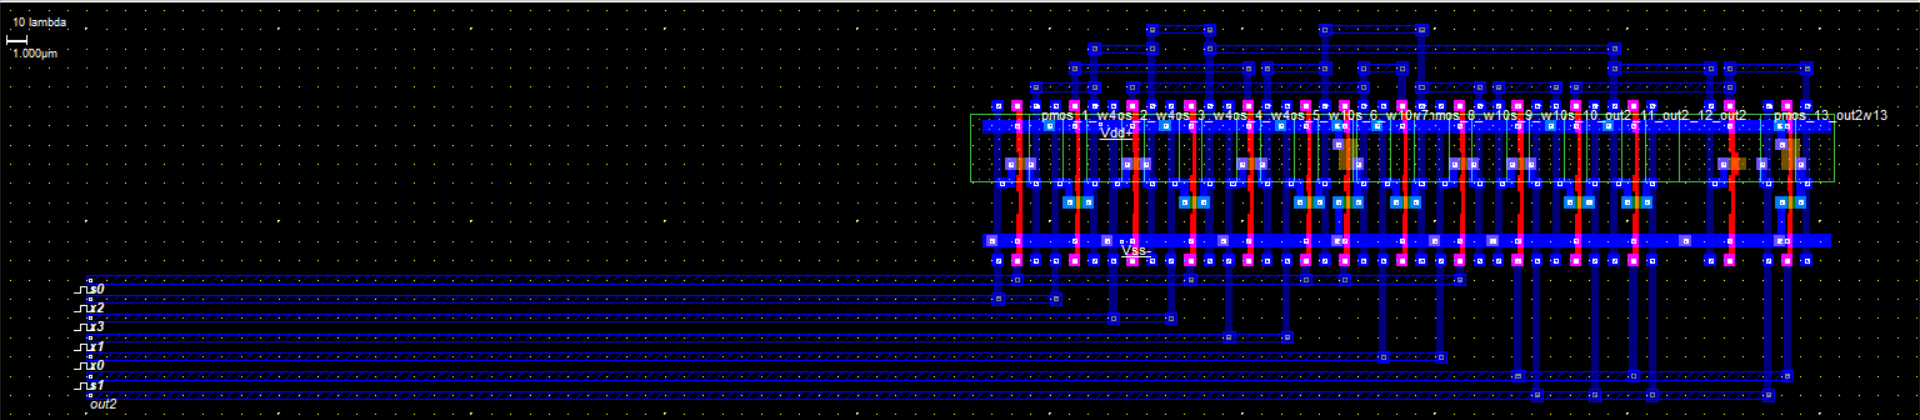
\includegraphics[scale = 0.40]{mwlayout.png}
    \caption{Layout generated by Microwind}
\end{figure} \newline
The silicon area occupied by this layout is found to be 1777.7 $\mu \text{m}^2$ which is considerably larger than the area that is occupied by the layout shown in Figure \ref{fig2}. The power consumed is also found to be 0.141mW which is significantly higher than the power consumed by the previous layout design.
In addition to this, the output waveform is also seen to incorporate more noise and propagation delay. Considering these factors, we have decided to choose Figure \ref{fig2} as the final layout design for the given problem statement

\newpage

\section {Problem 2}

\begin{tcolorbox}
    Design a modulo-6 counter, which counts in the sequence 0, 1, 2, 3, 4, 5, 0, 1$\cdots$. The counter counts the clock pulses if its enable input, E, is equal to 1. Use D flip-flops in your circuit.
\end{tcolorbox}

\subsection{Solution}
\subsubsection{Schematic design}
The schematic design is shown below
\begin{figure}[ht]
    \centering
    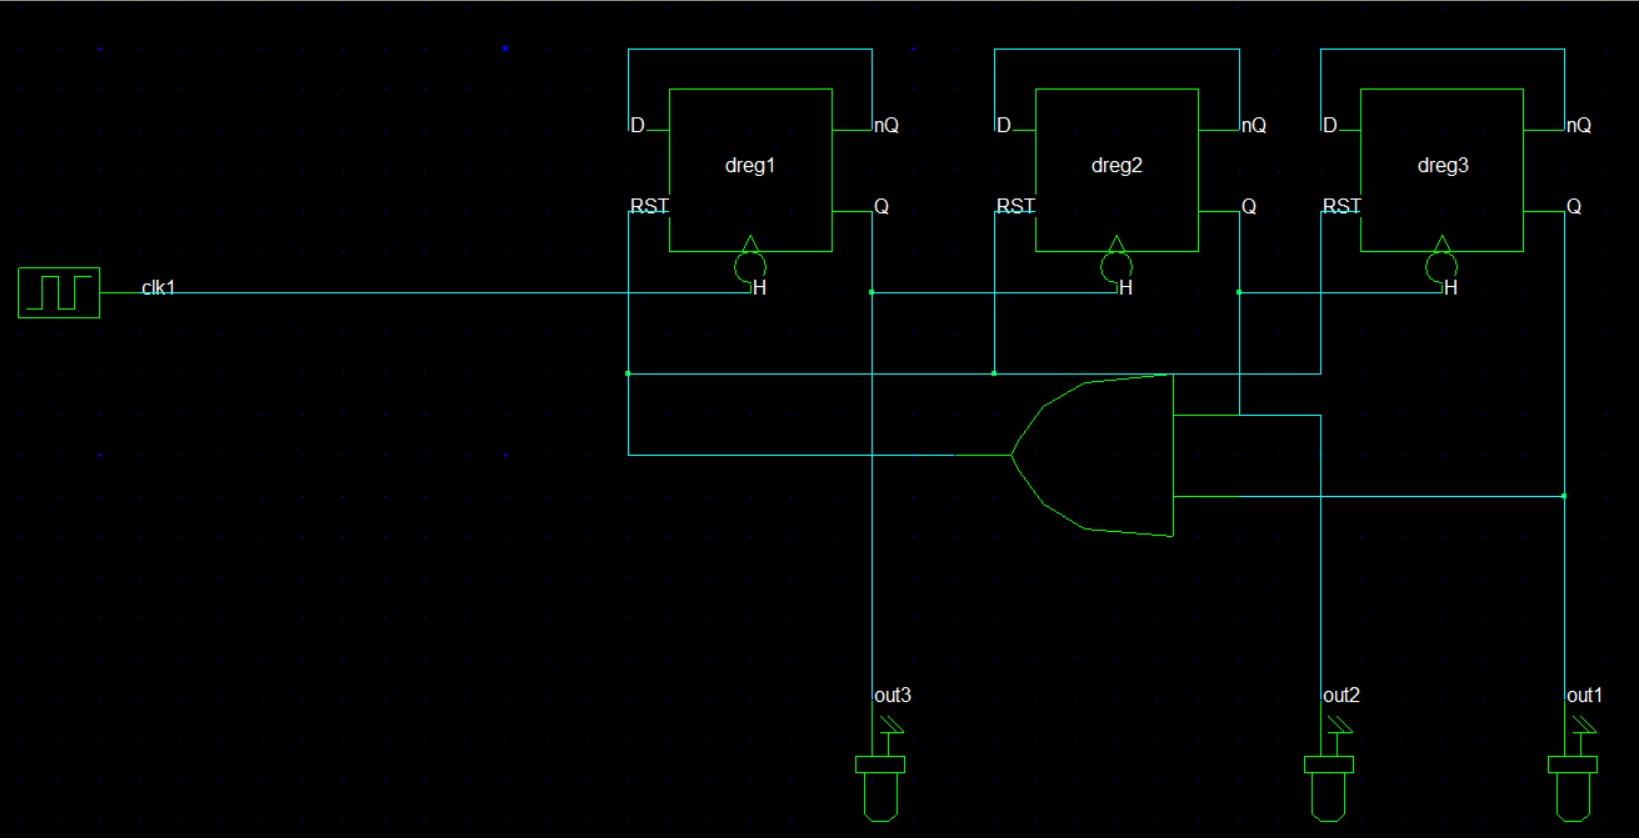
\includegraphics[scale = 0.4]{dff_sch.png}
    \caption{Schematic design for a mod 6 counter}
\end{figure}
\newpage
\subsubsection{Verilog Code}

\begin{lstlisting}[style={verilog-style}]
    module counter ( clk ,reset ,dout, enable );

        output reg [2:0] dout ;

        input wire clk ;
        input wire reset ;
        input wire enable;

        initial dout = 0;

        always @ (posedge (clk)) begin
            if (reset)
                dout <= 0;
            else if (dout<5 && enable ==1)
                dout <= dout + 1;
            else
                dout <= 0;
        end
endmodule
\end{lstlisting}

\subsubsection{Testbench}
\begin{lstlisting}[style={verilog-style}]
    module counter_tb();
    reg clk;
    reg reset;
    wire[2:0] out;
    reg enable;  
    counter c1(.clk(clk),.reset(reset),.dout(out),.enable(enable));
    always #10 clk = ~clk;
    initial begin
        enable = 0;
        #50 ; enable  = 1;
        {clk,reset}<=0;
    end      
endmodule
\end{lstlisting}
\newpage
\subsubsection{Output waveform}
\begin{figure}[ht]
    \centering
    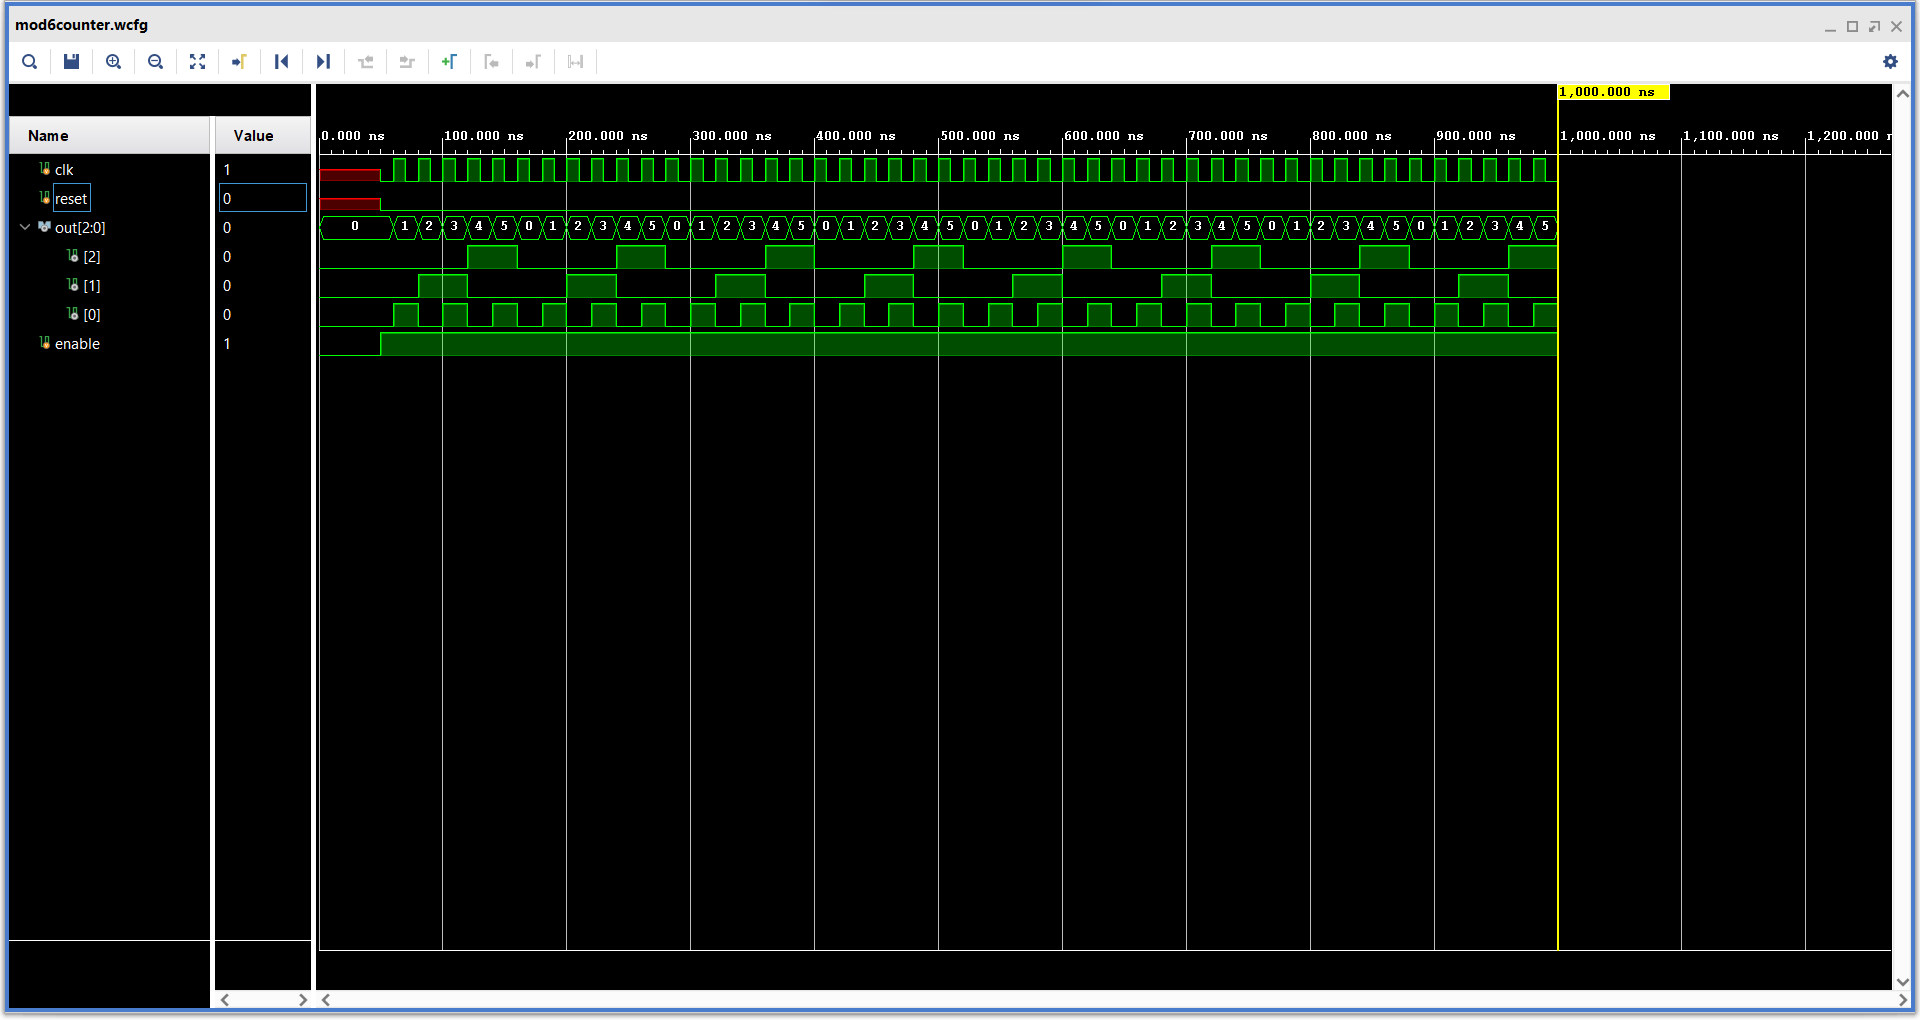
\includegraphics[scale = 0.4]{waveform.png}
    \caption{Output waveform of the counter}
\end{figure}
\end{document}
